\chapter{Grundlagen}
\label{chap:grundlagen}

\section{Technische Vorraussetzungen}
Eine Erläuterung und Erklärung der technischen Grundlagen, der beiden zentralen, verwenden Konzepten, das Aloha Protokoll und das Stromnetz sowie auf die Grundlagen von Elektrofahrzeugen.
\subsection{Aloha-Protokoll}
Das Aloha Protocol wurde an der Universität von Hawaii entwickelt. Ursprünglich wurde es dort für Übertragungen zwischen Funkstationen entwickelt, allerdings lässt sich das Protokoll überall dort verwenden, wo unkoordinierte Benutzer mit einem geteilten Medium arbeiten \cite{Back_AlohaPure}. Ein Vorteil des Aloha Protokolls liegt in seiner Einfachheit, die mit dem Netz verbunden Parteien senden ihre jeweiligen Datenpakete unabhängig der sonstigen Aktivität auf der Datenleitung. Die Übertragung gilt dann als erfolgreich, wenn eine Bestätigung erhalten wurde. Während der Übertragung lauscht jeder Teilnehmer auf die gesendete Information, somit bemerkt auch jeder Teilnehmer eine eventuell auftretende Kollision \cite{Back_AlohaPure}. Eine Kollision im Zusammenhang mit dem Aloha Protokoll bedeutet, dass mehr als ein Datenpaket gleichzeitig über die Datenleitung gesendet wurde. Diese Datenpaket haben sich an einem gewissen Punkt überlagert und es kann nicht festgestellt werden, welche Information zu welchem Paket gehört, weshalb alle Informationen verworfen werden und beide Pakete komplett neu gesendet werden müssen. \\
\begin{figure}[h!]
	\begin{center}
	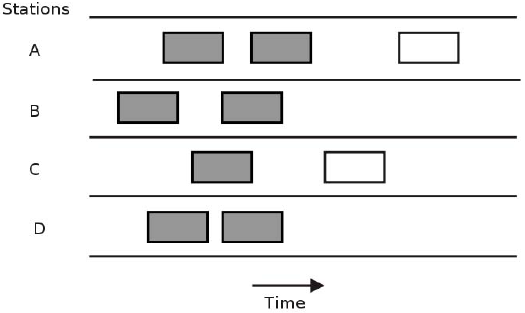
\includegraphics[width=\linewidth]{img/pureAloha.png}
	\caption{Datenübertragung mit Kolisionen unter Verwendung des Aloha Protokolls}
	\end{center}
	\label{Abb2_PureAloha}
\end{figure}
In der Abbildung \ref{Abb2_PureAloha} sind insgesamt neun Kästchen, sieben in grau und 2 in weiß, aufgeteilt auf die horizontalen Kanäle A bis D entlang einer unbeschrifteten Zeitachse verteilt. Die grau dargestellten Kästchen überschneiden sich immer mindesten zwei anderen grauen Paketen, diese Überschneidung entlang der Zeitleiste symbolisiert eine Kollision. Diese Tatsache erklärt, warum die beiden Kästchen ganz rechts andersfarbig, weiß, dargestellt sind, diese Kästchen überschneiden sich mit keinem anderen Kästchen. Da keine Überlagerungen aufgetreten sind, wurden diese Pakete erfolgreich übertragen. Aus Abbildung \ref{Abb2_PureAloha} wird ebenfalls ersichtlich, wie im Aloha Protokoll auf Kollisionen reagiert wird, die wachsenden Abstände zwischen Paketen von A, nachdem Pakete nicht erfolgreich gesendet wurden. Da eine Kollision bedeutet, dass mehr als eine Partei Dateien senden möchten, versucht man durch eine Wartezeit zu erreichen, das bei Ablauf der Wartezeit, die anderen Parteien ihre Daten bereits übertragen haben und so bei der eigene Übertragung keine Kollision mehr auftritt.\\
Eine Variante des Aloha Protokolls teilt die Zeit nun Schrittweise ein. In jedem dieser Zeitschritte kann ein Datenpaket gesendet werden. Die Länge dieser Zeitschritt muss global für alle mit dem Netzwerk verbunden Parteien gleich sein. Durch die Einteilung der Zeit in feste Abschnitte ist es nun nicht mehr möglich jederzeit mit dem Senden von Daten zu beginnen, dies ist nur möglich, wenn ein auch ein Zeit Abschnitt beginnt. Durch diese Einschränkungen in Zeitabschnitte und beim Beginn der Datenübertragung steigert sich die Effizienz des Protokolls und die Wahrscheinlichkeit für Kollisionen wird reduziert \cite{Back_AlohaPure}.

\subsection{Aufbau des Stromnetz}
Bei dem deutschen Stromnetz handelt es sich um ein Wechselspannungsnetz mit einer Normfrequenz von 50 Hz. Das Stromnetz in Deutschland lässt sich in vier Ebenen unterteilen.
\begin{figure}[h!]
	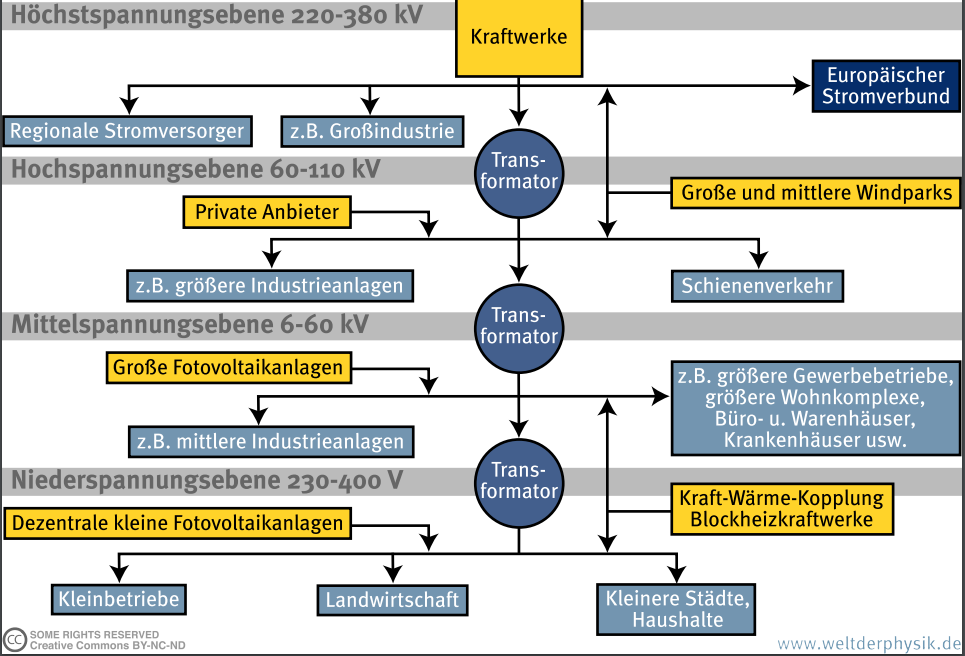
\includegraphics[width=\linewidth]{img/Stromnetz1.png}
	\caption{Aufbau des Stromnetzes}
	\label{Abb1_Stromnetz}
\end{figure}


Wie man an Hand des Bildes erkennen kann, unterscheiden sich die vier Ebenen vor allem anhand der verwendeten Spannung. Die im Bild gelb dargestellten Kästchen, beinhalten die Teilnehmer am Netz, welche nur Leistung einspeisen. Aus dem Bild wird ebenfalls klar, da sich auf allen Ebenen gelbe Kästchen befinden auch in jeder Ebene des Netzes Leistung entsprechender der jeweiligen Ebene eingespeist wird. An den drei Übergangspunkten zwischen der vier Schichten befinden sich sogenannte Transformatoren, dargestellt in blau. Diese sind in der Lage die eingehende Spannung, abhängig von der Windungszahl der in Ihnen verbauten Spulen zu erhöhen, in eine, von der Eingangsspannung verschiedene, Spannung umzuwandeln. Durch diese Fähigkeit agieren sie als Verbindungselement der verschiedenen Spannungsebenen, ebenso limitiert die Leistungsfähigkeit des Transformators die Leistungsfähigkeit des an Ihm angeschlossen Netzes bzw. Teilnetzes.
Im europäischen Staatenverbund sind die Stromnetze der aneinandergrenzenden Mitgliedsländer verbunden. Aus dem Schaubild wird ersichtlich, dass diese Verbindung auf der höchsten Spannungsebene erfolgt, dargestellt in dunkelblau .Die mit dem Stromnetz verbunden Abnehmer des Stroms werden in hellblau dargestellt, je nach dem auf welcher Eben des Netzes sie angesiedelt sind unterscheidet sich ihr Leistungsbezug. Dieser Unterschied wird auch aus den Bezeichnungen deutlich (Großindustrie, größere Industrie, mittlere Industrieanlagen, Kleinbetriebe). \\
Eine dieser Schichten wird nun genauer betrachtet und zwar die unterste, die Niederspannungsebene. Auf dieser Ebene befinden sich unter anderem die einzelnen Haushalte, mit ihren einzelnen Anschlüssen. Niederspannungsnetze in Deutschland sind meist sternförmig aufgebaut mit dem versorgenden Transformator am Mittelpunkt des Sternes gelegen. In diesem sternförmigen Aufbau gibt es nur einen Weg von Transformator zu einem bestimmten Verbraucher. Nur in den wenigsten Fällen wird von dem radialen Aufbau abgewichen und es erfolgt ein Mesh-artiger Aufbau des Netzes, in welchem dann auch mehr als nur ein Weg vom Transformator zu einem bestimmten Verbraucher geben kann. Die Leitungen eines Niederspannungsnetzes sind in Regel zwischen einigen 100 Metern und wenigen Kilometern lang, ja nach Verteilung der Anschlüsse. \\

Nachdem nun das Stromnetz vorgestellt wurde, wird nun noch auf den Strom selbst eingegangen, welcher mithilfe des Stromnetzes transportiert wird. Der Strom, bzw. der elektrische Strom, kann als sich bewegenden geladen Teilchen entlang eines Leiters verstanden werden, wobei das Stromnetz in diesem Fall als Leiter dient. Der elektrische Strom hängt von drei Faktoren ab, der verwendeten Spannung (U), Stromstärke(I) und dem vorherrschenden Widerstand (R). Diese drei Faktoren spielen eng dabei zusammen, wie viel Energie in Form von Strom übertragen werden kann. Die erste Einheit, die Spannung, steht für die Stärke, mit der der Strom transportiert wird, die Stromstärke für die Menge an geladen Teilchen, die pro Zeiteinheit transportiert werden und der Widerstand gibt an, welche Spannung nötig ist eine gewisse Stromstärke bei der Durchquerung eines Leiters aufrecht zu erhalten.(Scheinleistung/Blindleistung).

\subsection{Grundlagen zu Elektrofahrzeugen}
Ein Elektrofahrzeug ist ein Kraftfahrzeug, welches die für die Fortbewegung nötige Energie aus einem Akku bezieht, welcher zuerst aufgeladen werden muss. Die Energie die in diesem Akku gespeichert ist wird im Fahrzeug mit Hilfe von einem oder mehrere Elektromotoren in für die Fortbewegung des Fahrzeuges nutzbare Energie umgewandelt. Ein Elektrofahrzeug ist ein vielen Punkten ähnlich zu einem herkömmlichen Fahrzeug mit Verbrennungsmotor, was daran liegt, das nur die verwendete Energieform, deren Umwandlung in unmittelbar nutzbare Energie, sowie die Zuführung der verwendeten Energie zum Fahrzeug unterschiedlich sind. Ein Elektrofahrzeug verwendet elektrischen Strom zur Fortbewegung, dieser muss zuvor in das Fahrzeug geladen werden. Dieser Ladevorgang erfordert eine Verbindung des Elektroautos mit dem Stromnetz, diese Verbindung erfolgt über ein Ladegerät. Solche Ladegräte gibt es in verschieden Leistungsstufen von 2,5 kW bis 43 kW, je nach verwendeter Ladeleistung und Kapazität des Akkus variiert die benötigte Ladedauer ausgehenden vom jeweils aktuellen Ladestand des Fahrzeugs.

\section{Verfügbare Daten}
\label{cap:background_sec:setting}
Nun wird die Herkunft der für die nächsten Kapitel elementaren Daten erläutert. Ein Elektrofahrzeug verfügt über folgende Daten, die Ankunftszeit an der Ladestation für den aktuellen Ladezyklus, die Abfahrtszeit, wenn diese erreicht ist endet der aktuelle Ladezyklus. Ebenso gibt jedes Fahrzeug für sich an, ob es gerade verfügbar ist, sprich mit einer Ladestation verbunden ist, welchen Ladezustand der im Fahrzeug verbaute Akku aktuell hat, sowie die aktuell mögliche Ladeleistung. Die Ladegräte wissen jeweils welche Leistung sie gerade an das mit ihnen verbunden Elektrofahrzeug abgeben, sofern den ein Elektrofahrzeug mit ihnen verbunden ist. Einige Daten sind auch aus dem Stromnetz an sich bekannt, so ist die Leistungsabgabe des Transformators ans Stromnetz bekannt, sowie für jeden betrachten Hausanschluss, das dort aktuell vorherrschende Spannungslevel.

\section{VDE-Controller}
\label{cap:background_sec:pureVDE}
Die aktuell im Stromnetz vorliegende Situation, wird durch die Verwendung des Anschlusses ans Stromnetz gemäß der Technischen Anschlussregel Niederspannung(VDE-AR-N 4100) simuliert. Die Anschlussregel gibt vor, wie sich die aktuell anliegende Spannung auf den möglichen Leistungsbezug des Anschlusses auswirkt. \\
\begin{figure}[h!]
	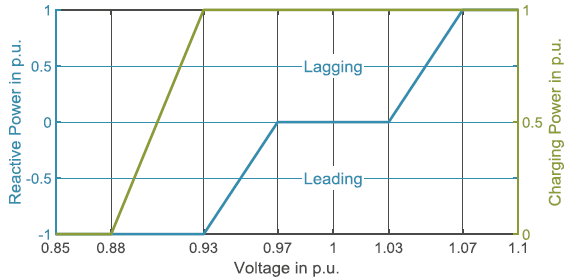
\includegraphics[width=\linewidth]{img/VDEGraph.png}
	\caption{Spannungs zu Leistungsverhältnis nach VDE-AR-N 4100(grün)}
	\label{Abb_VDEController}
\end{figure}
Per Definition wird von einer Normspannung von 230 Volt ausgegangen. Aus der Abbildung \ref{Abb_VDEController} ist erkennbar, dass wenn weniger als 93\% dieser Normspannung vorliegen, wird die Leistung linear reduziert, wenn der Wert der anliegenden Spannung unter 88\% der Normspannung fällt, wird der Leistungsbezug komplett eingestellt, bis die Spannung wieder auf mindestens 88\% der Normspannung von 230 Volt steigt. Bei einer Spannung zwischen 93\% und 88\% der Normspannung wird der mögliche Leistungsbezug, in diesem Fall die Ladeleistung, linear von voller geforderter Leistung bis zur Abschaltung reduziert.\\
Bis auf die Leistungsreduktion werden von dieser Anschlussregel keine weiteren Maßnahmen getroffen um die Spannung im Netz stabil zu halten. 
Neben der Leistungsreduktion ist es ebenfalls möglich Blindleistung wieder in Stromnetz einzuspeisen um Das Spannungslevel zu erhöhen(Siehe Abbildung \ref{Abb_VDEController}, blaue Kurve), diese Möglichkeit wird aber nicht weiter betrachtet.

\section{Slotted Aloha, Wartezeit nur über Teilnehmer}
\label{cap:background_sec:SA_participants}
Diese Art der Verwendung des Slotted ALOHA Protokolls, definiert eine Kollision, wenn der aktuell vorliegende Spannungswert unter 93\% der Normspannung von 230 Volt fällt. Tritt eine Kollision auf, wird die aktuell anliegende Leistung auf Null reduziert und eine Wartezeit bestimmt, in welcher keine Leistung aus dem Netz bezogen wird. Die Wartezeit wird per Zufall bestimmt, sie wird aus einem Intervall gezogen. Dieses Intervall beginnt  bei Null und wird nach oben von der aktuell Anzahl an Fahrzeugen begrenzt, welche aktuell mit einer beliebigen im Netz installierten Ladestation verbunden sind. Nach dem Ablauf der Wartezeit wird wieder Leistung aus dem Netz bezogen, bis entweder keine Leistung mehr benötigt wird oder wieder eine Kollision auftritt.
Bei dieser Art der Bestimmung der Wartezeit wird weder der aktuelle Ladezustand, noch die verbleibende Zeit des Fahrzeuges am Ladegerät bis zur nächsten Abfahrt berücksichtigt. Lediglich die Zahl der aktuell mit dem Netz verbunden Fahrzeuge, egal ob ladend, wartend oder bereits fertig geladen, wird berücksichtigt.

